\documentclass[11pt]{IEEEtran}

\usepackage{graphicx}
\usepackage[style=ieee,backend=bibtex8]{biblatex}
\bibliography{bibliography}

\begin{document}

\title{Towards a Self Guided Team Based eLearning Solution}

\author{D.~K.~Allison,~J.~Harty}

\maketitle

\markboth{Towards Self Guided ELearning}{}

\begin{abstract}
Millions of learners have little chance of success in terms of personal 
development globally, the schools are missing some of the teachers, they have 
very few resources and the teaching is rote-based. eLearning has been touted as 
one way to compensate for the lack of teachers and the lack of other learning
resources, however there's patchy evidence that the currently available 
resources materially help the pupils learn skills that matter. Also the 
materials may not be particularly suited to the level, or learning syles of the 
pupils. Also the materials may be very relevant to the location, language, or 
context of the school.

This position paper captures the essence of an elearning system which may help 
to address many of the concerns, and be viable in environments and contexts were
there are few trained teachers available. It supports team-based learning where 
the learners have to be able to work unaided for extended periods. The paper 
also explores whether and how differences in the skill levels of participants 
can be used to improve the learning, and whether the pairings (etc) break down 
if there are large differences between the skill levels of the participants. In 
some cases, algorithms may be able to detect common-modes of mistakes, such as 
where learners mistakenly believe 0 - any number = 0 and pair that learner with 
someone who understands the correct approach to solving this problem so that 
pupils help each other to learn and develop their skills.

It may also be suitable and relevant for situations and contexts where there are
more, and more competent teachers, and better resources and facilities 
available. The authors are interested in designing and devising a reference
implementation available as opensource software with materials available under
permissive sharing licenses such as creative commons.
\end{abstract}

\begin{IEEEkeywords}
Holography, image analysis.
\end{IEEEkeywords}

% Main section includes
\section{Objectives}

\begin{itemize}
\item Support partially or unguided learning.
\item Support classification of assessment failures.
\item Support tree based learning patterns.
\item Support creation of balanced learning teams.
\item Support teacher assessment of learning needs in real time.
\item Gather compelling evidence using metrics of progress
\end{itemize}



% Include all citations in the database
\nocite{*}

% Some example resources
\section{Examples}

\begin{figure}[t]
\centering
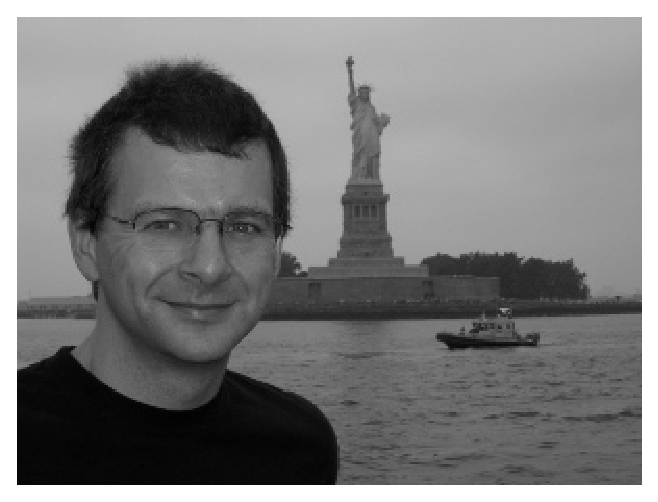
\includegraphics[width=200px]{figures/julian-harty.eps}
\caption{(a) Diagram of the experimental set up. (b) Detail of the test object used.}
\label{fig_env1}
\end{figure}

\begin{equation}
x=\sum\limits_{1=0}^z 2^1Q
\label{eq1}
\end{equation}%

\begin{table}[!t]
\centering
\caption{Math Spacings Used By \LaTeX}
\label{tab1}
\begin{IEEEeqnarraybox}[\IEEEeqnarraystrutmode\IEEEeqnarraystrutsizeadd{2pt}{1pt}]{v/c/v/r/v/c/v/c/v/c/v}
\IEEEeqnarrayrulerow\\
& \mbox{{\bf Size}} && \mbox{{\bf Width}} && \mbox{{\bf Cmd.}} &&
\mbox{{\bf Used for}} && \mbox{{\bf Example}} &\\
\IEEEeqnarraydblrulerow\\
\IEEEeqnarrayseprow[3pt]\\
& \mbox{small} && \mbox{1/6 em} && \verb+\,+ && \mbox{symbols} && a b &\IEEEeqnarraystrutsize{0pt}{0pt}\\
\IEEEeqnarrayseprow[3pt]\\
\IEEEeqnarrayrulerow\\
\IEEEeqnarrayseprow[3pt]\\
& \mbox{medium} && \mbox{2/9 em} && \verb+\:+ && \mbox{binary operators} && a + b &\IEEEeqnarraystrutsize{0pt}{0pt}\\
\IEEEeqnarrayseprow[3pt]\\
\IEEEeqnarrayrulerow\\
\IEEEeqnarrayseprow[3pt]\\
& \mbox{large} && \mbox{5/18 em} && \verb+\;+ && \mbox{relational operators}&& a = b &\IEEEeqnarraystrutsize{0pt}{0pt}\\
\IEEEeqnarrayseprow[3pt]\\
\IEEEeqnarrayrulerow\\
\IEEEeqnarrayseprow[3pt]\\
& \mbox{negative small} && \mbox{${-}$1/6 em} && \verb+\!+ && \mbox{misc. uses} && ab &\IEEEeqnarraystrutsize{0pt}{0pt}\\
\IEEEeqnarrayseprow[3pt]\\
\IEEEeqnarrayrulerow
\end{IEEEeqnarraybox}
\end{table}

\begin{itemize}
\item Weight parameters for the simulated robot.
\item Length of each body link.
\item Specifications of body joints. Upper Torso means the spine. Due to symmetry, body parts from the right are not shown.
\item Neuron parameters. $\Theta$ is the threshold, $\Gamma$ is the gain. $\tau_{D}$ and $\tau_{A}$ are respectively the time constant of the dendritic sums and that of the frequency adaptation. $\mu$ is the coefficient of frequency adaptation.
\end{itemize}
Holograms recorded in such a fashion can not be reconstructed in the conventional way with an optical reconstruction beam. In order to numerically reconstruct the holograms, the surface modulation was digitized with a Novascan atomic force microscope (AFM) operated in tapping mode. Holograms recorded in such a fashion can not be reconstructed in the conventional way with an optical reconstruction beam. In order to numerically reconstruct the holograms, the surface modulation was digitized with a Novascan atomic force microscope (AFM) operated in tapping mode. 
\begin{enumerate}
\item Screenshot of the Webots simulation environment.
\item Schematic diagram of the simulated robot.
\item Schematic of the model lamprey CPG. Connections with a dot ending represent inhibitory connections while those with an arrow ending represent excitatory connections.
\item Sample output of a segmental oscillator (the 20th segment from the CPG). MNl and MNr respectively represents the output from the left and right motoneurons. Note the regularity of the neural pulses.
\end{enumerate}

% A non numbered section
\section*{Acknowledgements}
The authors wish to thank the anonymous reviewers for their valuable suggestions.

\printbibliography

\end{document}



